\documentclass[tikz,border=4pt]{standalone}
\usepackage{amsmath}
\usetikzlibrary{patterns}
\begin{document}
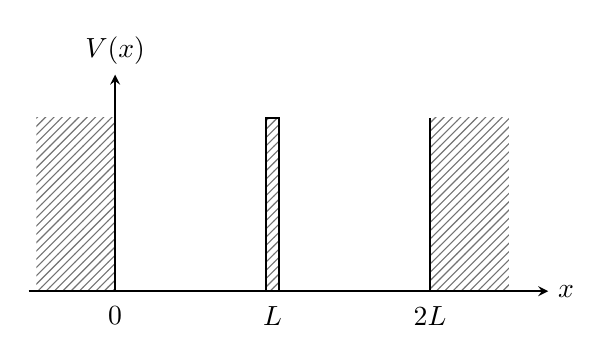
\begin{tikzpicture}[>=stealth, thick, scale=1.0]
  % Hatched walls: x < 0, thin barrier at x = L (x=2.0), and x > 2L (x=4.0)
  \fill[pattern=north east lines, pattern color=black!55] (-1.0, 0) rectangle (0, 2.2);
  \fill[pattern=north east lines, pattern color=black!55] (1.92, 0) rectangle (2.08, 2.2);
  \fill[pattern=north east lines, pattern color=black!55] (4.0, 0) rectangle (5.0, 2.2);

  % Wall outlines
  \draw[line width=0.85pt] (0, 0) -- (0, 2.2);
  \draw[line width=0.85pt] (1.92, 0) -- (1.92, 2.2) -- (2.08, 2.2) -- (2.08, 0);
  \draw[line width=0.85pt] (4.0, 0) -- (4.0, 2.2);

  % Axes
  \draw[->, line width=0.6pt] (-1.1, 0) -- (5.5, 0) node[right] {$x$};
  \draw[->, line width=0.6pt] (0, 0) -- (0, 2.75) node[above] {$V(x)$};

  % Ticks
  \node[below] at (0, -0.06) {$0$};
  \node[below] at (2.0, -0.06) {$L$};
  \node[below] at (4.0, -0.06) {$2L$};
\end{tikzpicture}
\end{document}
